% !LW recipe=xelatex-bibtex
% Build: xelatex main, bibtex main, xelatex main, xelatex main (the recipe is in .vscode/settings.json).
% Same template as the customer-churn-prediction report.
\documentclass[a4paper,11pt]{report}

% ---- Page layout ----
\usepackage[margin=2.5cm]{geometry}

% ---- Fonts (XeLaTeX; needed for correct Vietnamese diacritics) ----
\usepackage{fontspec}

% ---- Typography & links ----
\usepackage{microtype}
\usepackage[dvipsnames]{xcolor}
\usepackage{hyperref}
\hypersetup{
    colorlinks = true,
    linkcolor  = blue!50!black,
    citecolor  = blue!50!black,
    urlcolor   = blue!50!black,
    pdftitle   = {Merging Five GLUE NLP Tasks Using Weight-Ensembling Mixture of Experts},
    pdfauthor  = {Nguyễn Bá Anh; Phạm Nguyên Đăng}
}

% ---- Math ----
\usepackage{amsmath,amssymb,mathtools}

% ---- Figures & tables ----
\usepackage{graphicx}
\usepackage{float}
\usepackage{booktabs}
\usepackage{array}
\usepackage{tabularx}
\usepackage{caption}
\usepackage{subcaption}
\usepackage{tikz}
\graphicspath{{figures/}}
% Shared TikZ styles: NavyBlue comes from the report theme; the colour roles are constant across figures.
\usetikzlibrary{arrows.meta,fit,backgrounds,calc,positioning}
\tikzset{
  every node/.append style={font=\footnotesize\linespread{1}\selectfont},
  box/.style={rounded corners=1.5pt,align=center,inner sep=2.5pt,minimum height=.75cm},
  frz/.style={box,draw=NavyBlue,fill=NavyBlue!8},
  mix/.style={box,draw=BurntOrange,fill=Goldenrod!25,thick},
  trn/.style={box,draw=BrickRed,fill=BrickRed!14,thick},
  dat/.style={box,draw=black!50,fill=black!5},
  plain/.style={box,draw=none,fill=none},
  flow/.style={-{Latex[length=2mm]},thick,black!80},
  gate/.style={-{Latex[length=2mm]},thick,BrickRed},
  dict/.style={-{Latex[length=2mm]},thick,NavyBlue},
  group/.style={rounded corners=3pt,draw=black!45,dashed,inner sep=5pt},
  note/.style={font=\scriptsize\linespread{1}\selectfont,text=black!75,align=center},
  lane/.style={font=\footnotesize\bfseries,text=NavyBlue,anchor=west}
}
\newcommand{\figlegend}{%
  {\scriptsize\tikz\node[frz,minimum height=.22cm,minimum width=.35cm,inner sep=0]{};~frozen\quad
  \tikz\node[mix,minimum height=.22cm,minimum width=.35cm,inner sep=0]{};~input-conditioned\quad
  \tikz\node[trn,minimum height=.22cm,minimum width=.35cm,inner sep=0]{};~trainable during FSFT}}


% ---- References ----
\usepackage[numbers,sort&compress]{natbib}
\usepackage{url}

% ---- Header / footer ----
\usepackage{fancyhdr}
\pagestyle{fancy}
\fancyhf{}
\rfoot{\thepage}
\renewcommand{\headrulewidth}{0pt}

% ---- Macros used by the chapters and figures ----
% Compact type for tables
\newcommand{\tablestyle}{\footnotesize\renewcommand{\arraystretch}{1.12}\setlength{\tabcolsep}{4.5pt}}
% Small type inside TikZ figures
\newcommand{\figfont}{\fontsize{7}{8.4}\selectfont}
\hyphenation{WEMoE GLUE BERT}
\renewcommand{\bibname}{References}

\begin{document}

\begin{titlepage}
    \centering
    \vspace*{3cm}

    {\LARGE\bfseries Merging Five GLUE NLP Tasks Using\\Weight-Ensembling Mixture of Experts}\\[0.4cm]
    {\Large Few-Shot Router Training on a Shared BERT Backbone}\\[2cm]

    \rule{0.8\linewidth}{0.6pt}\\[0.5cm]
    {\large Introduction to Deep Learning}\\[0.2cm]
    \rule{0.8\linewidth}{0.6pt}

    \vfill

    \begin{tabular}{ll}
        \textbf{Instructor:} & Trần Việt Trung \\
    \end{tabular}

    \vspace{0.8cm}

    \textbf{Group Members}\\[0.3cm]
    \begin{tabular}{ll}
        Nguyễn Bá Anh & 20261218M \\
        Phạm Nguyên Đăng & 20261209M \\
    \end{tabular}

    \vspace{1cm}
    {\large Hanoi University of Science and Technology}\\[0.3cm]
    {\large \today}

    \vspace*{1cm}
\end{titlepage}

\tableofcontents

\chapter*{Abstract}
\addcontentsline{toc}{chapter}{Abstract}
\markright{Abstract}
Fine-tuning one pre-trained language model per task gives strong task-specific performance, but every new task adds a complete model to train, store and serve, and nothing learned for one task reaches the others. This study examines whether several fine-tuned models can become a single multi-task model whose weights adapt to the input. We adapt Weight-Ensembling Mixture of Experts (WEMoE), previously evaluated on vision Transformers, to BERT and five binary tasks of the GLUE benchmark: MRPC, RTE, CoLA, SST-2 and QNLI. Weights outside the MLP blocks are merged statically with Task Arithmetic, while the MLP weights of every encoder layer are rebuilt for each input as the pre-trained weights plus a router-weighted sum of frozen task vectors. Only the routers are trained, by Few-Shot Fine-Tuning (FSFT) on labelled examples that the experts never saw. All model selection uses a development split, and scores are reported on the official validation splits. With 256 examples per task, WEMoE reaches an average score of $69.9\pm0.1$, against 57.4 for Task Arithmetic, 78.2 for the experts and 45.8 for a majority-class predictor, which is 59.1\% of the gain between the majority class and the experts. Coefficients that do not depend on the input reach only $58.4\pm0.0$. Upscaling only the first MLP layer gives a similar average ($69.1\pm0.1$) with 47.2\% of the storage of five experts rather than 73.1\%, but the two variants are weak on different tasks. WEMoE matches the experts on no task and is several times slower in batches. Limitations include a single set of experts, small validation sets for two tasks, and development data that exceeds the few-shot budget.

\vspace{3mm}
\noindent\textbf{Keywords:} model consolidation; weight ensembling; Mixture of Experts; BERT; multi-task learning; few-shot fine-tuning.


\chapter{The Problem}
\label{ch:problem}
\section{Why One Separate Model per Task Does Not Scale}

Pre-trained language models have changed how natural language processing systems are built. An encoder such as BERT~\cite{devlin2019bert} can be fine-tuned for a new classification problem with limited data, so a system that supports several language understanding tasks tends to collect one fine-tuned copy of the same architecture per task. Each copy performs well on its own task, yet the collection becomes costly in four ways.

\begin{itemize}
  \item \textbf{Storage.} Every copy holds a complete parameter set, although all copies start from the same pre-trained weights.
  \item \textbf{Training.} Every new task requires another full fine-tuning run, with its own data, compute and model selection.
  \item \textbf{Serving.} A deployment must version, load and route requests to a separate model for each task.
  \item \textbf{Knowledge isolation.} Each model knows only its own task. Whatever it learned during fine-tuning is not available to the others.
\end{itemize}

\section{Problem Statement and Research Questions}
\label{sec:problem}

Let $\theta_0$ be the weights of a pre-trained model, and let $\theta_i$, $i\in\mathcal{T}$, be the weights of models fine-tuned from it for a set $\mathcal{T}$ of $T$ tasks. We call each fine-tuned model an \emph{expert}. The \emph{task vector} of task $i$ is the change that fine-tuning made to the shared starting point:
\begin{equation}
\tau_i=\theta_i-\theta_0 .
\label{eq:task-vector}
\end{equation}
The input of the problem is $\theta_0$ with the weights $\theta_i$, or equivalently with the task vectors. The output is one multi-task model with weights $\theta_{\mathrm{mer}}=C(\theta_0,\theta_i)$, which maps a text and its task to a label. The problem is to find a merge function $C$ such that the merged model meets three objectives:

\begin{enumerate}
  \item[\textbf{O1.}] It integrates task knowledge \emph{dynamically}, depending on the input.
  \item[\textbf{O2.}] It stays close to the quality of the task-specific models.
  \item[\textbf{O3.}] It needs fewer stored parameters than keeping all the models.
\end{enumerate}

No pass threshold was fixed in advance, so ``close'' is reported as a measured distance and not as a binary outcome. This study addresses four research questions:

\begin{enumerate}
  \item[\textbf{RQ1.}] How much of the performance lost by static merging can routers recover when they are trained on labelled examples that the experts never saw?
  \item[\textbf{RQ2.}] How does that recovery depend on the labelled budget?
  \item[\textbf{RQ3.}] Does the improvement require routing that depends on the input, or would better fixed coefficients be enough?
  \item[\textbf{RQ4.}] How does the choice of upscaled MLP layers affect per-task behaviour and storage, and what does the method cost at inference?
\end{enumerate}

\section{Why the Problem Matters and Why It Is Difficult}

\emph{Model consolidation}, the merging of already fine-tuned models into one, matters because many systems serve related language tasks and a shared model makes knowledge reusable across them. Multi-task learning~\cite{caruana1997multitask} also produces one model, but it trains jointly on all the data and repeats that cost when a task is added. Consolidation starts from models that already exist, so it needs no joint retraining from scratch.

The difficulty lies in how fine-tuned models disagree. Updates that help one task can harm another when they land on the same parameters, which is known as \emph{task interference}. Two models can also pull one weight in opposite directions, so that a sum partly cancels what each of them learned. Any merge must therefore decide how much of each update to keep, and it must do so without the original training data of every task.

\section{Why Static Merging Alone May Be Insufficient}

A static method such as Task Arithmetic~\cite{ilharco2023task} combines parameters once and commits to one set of weights for all inputs. The five tasks in this study make the limitation concrete. They differ in what they ask of the encoder: judging one sentence for grammar or sentiment, or relating two sentences through paraphrase, entailment or question answering. A single parameter vector must serve all of these at once, and its scaling factor can only trade them against one another. As Tang et al.~\cite{tang2024wemoe} argue, the best solution can vary with the input, so one fixed result is unlikely to be the best for every task. The gap this report examines is therefore whether merged weights should change with the input instead of staying fixed.


\chapter{The Idea}
\label{ch:idea}
\section{Mixture of Experts: The Core Concept}

A Mixture of Experts (MoE)~\cite{jacobs1991adaptive,shazeer2017moe,mu2025survey} solves a problem through several specialised networks $E_1,\dots,E_n$ and a small network called the \emph{router} or gate, $G$, which decides how much each expert counts for the current input (Figure~\ref{fig:moe}):
\begin{equation}
\mathrm{MoE}(x)=C\big(\{G_i(x)\cdot E_i(x)\}_{i=1}^{n}\big),
\label{eq:moe}
\end{equation}
where $G_i(x)$ is the contribution of expert $i$ and $C$ is a combination function, classically a sum. Because $G$ takes $x$ as its input, the contributions differ from one input to the next. This is the dynamic behaviour that objective O1 asks for.

\begin{figure}[htbp]
  \centering
  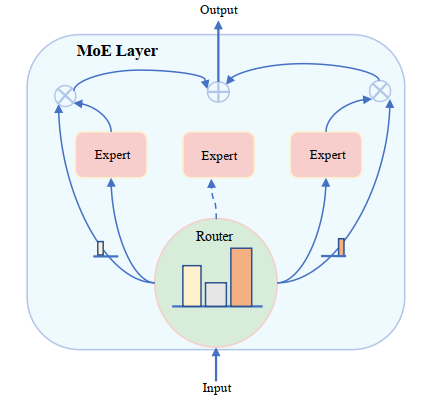
\includegraphics[width=.38\linewidth]{arch_moe.png}
  \caption{A Mixture of Experts layer, from Mu and Lin~\cite{mu2025survey}. The router sets the contribution of each expert for the current input.}
  \label{fig:moe}
\end{figure}

\section{From Output Ensembling to Weight Ensembling}

Equation~\eqref{eq:moe} combines expert \emph{outputs}. Applied directly, it would run every expert for every input, so inference cost would grow with the number of experts and the experts would need a shared output space. Weight-Ensembling Mixture of Experts (WEMoE)~\cite{tang2024wemoe} keeps the router but changes what is combined. An expert is represented by its task vector, the router's values scale those vectors, and the resulting weights are assembled before they are applied (Figure~\ref{fig:we}).

The two forms are not equivalent. For a single linear layer, $(\sum_i w_iW_i)h=\sum_i w_i(W_ih)$, but this equality is lost across non-linear activations and stacked layers. Weight ensembling therefore defines a different function from an ensemble of the experts' outputs. Its potential benefits are one forward pass per input, one checkpoint, and a shared encoder. Its costs are that task vectors must stay stored for every upscaled module, that routers need data to train, and that each input needs its own weights assembled at run time, which can make inference slower even when fewer parameters are stored. Section~\ref{sec:efficiency} measures these costs.

\begin{figure}[htbp]
  \centering
  \resizebox{.62\linewidth}{!}{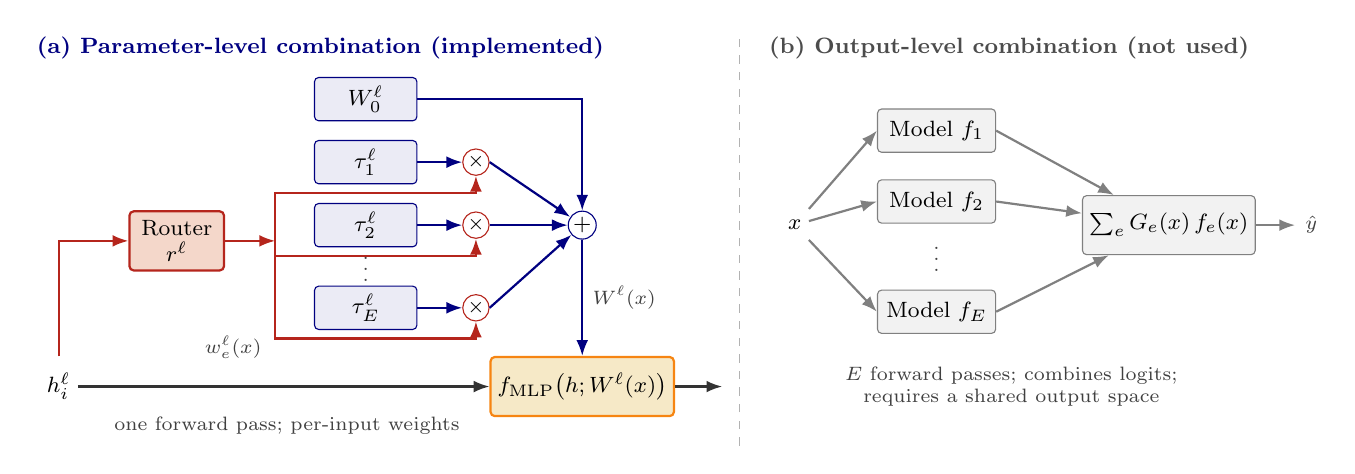
\begin{tikzpicture}[x=1cm,y=1cm]
  % (a) parameter-level: the gating weight of each expert scales its frozen task vector
  \node[lane] at (-.3,3.05) {(a) Parameter-level combination (implemented)};
  \node[plain] (h) at (.1,-1.25) {$h^{\ell}_i$};
  \node[trn,minimum width=1.2cm] (r) at (1.6,.6) {Router\\$r^{\ell}$};
  \draw[gate] (h.north) |- (r.west);
  \node[frz,minimum width=1.3cm,minimum height=.55cm] (w0) at (4.0,2.4) {$W_0^{\ell}$};
  \draw[gate] (r.east) -- (2.85,.6);
  \foreach \l/\y/\i in {$\tau_1^{\ell}$/1.6/1,$\tau_2^{\ell}$/.8/2,$\tau_E^{\ell}$/-.25/3}{
    \node[frz,minimum width=1.3cm,minimum height=.55cm] (t\i) at (4.0,\y) {\l};
    \node[circle,draw=BrickRed,inner sep=.5pt,font=\scriptsize] (x\i) at (5.4,\y) {$\times$};
    \draw[dict] (t\i) -- (x\i);
    \draw[gate] (2.85,.6) |- (5.4,\y-.39) -- (x\i.south);
  }
  \node[note] at (4.0,.34) {$\vdots$};
  \node[note,anchor=east] at (2.8,-.75) {$w^{\ell}_e(x)$};
  \node[circle,draw=NavyBlue,inner sep=.5pt] (s) at (6.75,.8) {$+$};
  \draw[dict] (w0.east) -| (s.north);
  \foreach \i in {1,2,3} \draw[dict] (x\i.east) -- (s);
  \node[mix,minimum width=2.3cm] (f) at (6.75,-1.25) {$f_{\mathrm{MLP}}\big(h;W^{\ell}(x)\big)$};
  \draw[dict] (s) -- node[note,right] {$W^{\ell}(x)$} (f);
  \draw[flow] (h) -- (f);
  \draw[flow] (f.east) -- ++(.6,0);
  \node[note] at (3.0,-1.75) {one forward pass; per-input weights};
  % (b) output-level
  \draw[black!30,dashed] (8.75,-2) -- (8.75,3.2);
  \node[lane,text=black!70] at (9,3.05) {(b) Output-level combination (not used)};
  \node[plain] (x) at (9.45,.8) {$x$};
  \foreach \l/\y/\i in {$f_1$/2.0/1,$f_2$/1.1/2,$f_E$/-.3/3}{
    \node[dat,minimum width=1.5cm,minimum height=.55cm] (m\i) at (11.25,\y) {Model \l};
    \draw[flow,black!50] (x) -- (m\i.west);
  }
  \node[note] at (11.25,.47) {$\vdots$};
  \node[dat,minimum width=1.75cm] (ls) at (14.2,.8) {$\sum_e G_e(x)\,f_e(x)$};
  \foreach \i in {1,2,3} \draw[flow,black!50] (m\i.east) -- (ls);
  \draw[flow,black!50] (ls.east) -- ++(.5,0) node[right,note] {$\hat y$};
  \node[note] at (12.2,-1.25) {$E$ forward passes; combines logits;\\requires a shared output space};
\end{tikzpicture}
}
  \caption{Parameter-level combination used in this study (a), contrasted with output-level combination (b), which is shown only for reference.}
  \label{fig:we}
\end{figure}

\section{Implementation Flow: From Datasets to Evaluation}
\label{sec:flow}

Figure~\ref{fig:flow} shows the implementation flow in four stages. Stage 1 prepares the five GLUE tasks and divides each official training split into three parts. Stage 2 fine-tunes one expert per task from the pre-trained model, then keeps its task vector and classification head. Stage 3 merges these into one model and trains its routers on the few-shot pool. Stage 4 reports scores on the official validation splits, together with storage and latency. The development split selects the best epoch, the scaling factor $\lambda$ and the best router step, so no selection touches the reported data. Expert weights stay frozen after Stage 2, and only the routers learn in Stage 3.

\begin{figure}[htbp]
  \centering
  \resizebox{.8\linewidth}{!}{% Four-stage flow of the Version 3 presentation (slide 11); theta_0 also feeds the merge, as in the code.
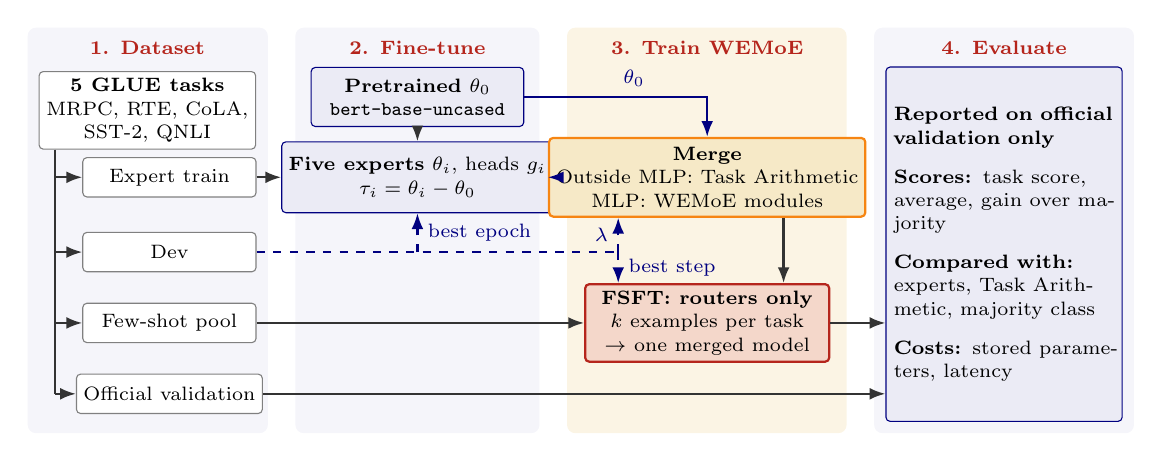
\begin{tikzpicture}[x=1cm,y=1cm]
  \fill[NavyBlue!4,rounded corners=3pt] (-.3,-2.65) rectangle (2.75,2.5);
  \fill[NavyBlue!4,rounded corners=3pt] (3.1,-2.65) rectangle (6.2,2.5);
  \fill[Goldenrod!12,rounded corners=3pt] (6.55,-2.65) rectangle (10.1,2.5);
  \fill[NavyBlue!4,rounded corners=3pt] (10.45,-2.65) rectangle (13.75,2.5);
  \node[font=\figfont\bfseries,text=BrickRed] at (1.22,2.25) {1. Dataset};
  \node[font=\figfont\bfseries,text=BrickRed] at (4.65,2.25) {2. Fine-tune};
  \node[font=\figfont\bfseries,text=BrickRed] at (8.33,2.25) {3. Train WEMoE};
  \node[font=\figfont\bfseries,text=BrickRed] at (12.1,2.25) {4. Evaluate};
  \node[dat,fill=white,minimum width=2.75cm,font=\figfont] (d) at (1.22,1.45) {\textbf{5 GLUE tasks}\\ MRPC, RTE, CoLA,\\ SST-2, QNLI};
  \node[dat,fill=white,minimum width=2.2cm,minimum height=.5cm,font=\figfont] (tr) at (1.5,.6) {Expert train};
  \node[dat,fill=white,minimum width=2.2cm,minimum height=.5cm,font=\figfont] (dv) at (1.5,-.35) {Dev};
  \node[dat,fill=white,minimum width=2.2cm,minimum height=.5cm,font=\figfont] (fs) at (1.5,-1.25) {Few-shot pool};
  \node[dat,fill=white,minimum width=2.2cm,minimum height=.5cm,font=\figfont] (va) at (1.5,-2.15) {Official validation};
  \draw[thick,black!80] (.05,1.45 |- d.south) -- (.05,-2.15);
  \foreach \n in {tr,dv,fs,va}{\draw[flow] (.05,0 |- \n.west) -- (\n.west);}
  \node[frz,minimum width=2.7cm,font=\figfont] (p) at (4.65,1.62) {\textbf{Pretrained} $\theta_0$\\ \texttt{bert-base-uncased}};
  \node[frz,minimum width=2.7cm,minimum height=.9cm,font=\figfont] (e) at (4.65,.6) {\textbf{Five experts} $\theta_i$, heads $g_i$\\ $\tau_i=\theta_i-\theta_0$};
  \draw[flow] (p) -- (e);
  \draw[flow] (tr.east) -- (e.west |- tr.east);
  \node[mix,minimum width=3.1cm,minimum height=1cm,font=\figfont] (m) at (8.33,.6) {\textbf{Merge}\\ Outside MLP: Task Arithmetic\\ MLP: WEMoE modules};
  \node[trn,minimum width=3.1cm,minimum height=.9cm,font=\figfont] (f) at (8.33,-1.25) {\textbf{FSFT: routers only}\\ $k$ examples per task\\ $\to$ one merged model};
  \draw[dict] (e.east) -- (m.west);
  \draw[dict] (p.east) -| node[pos=.3,above,font=\figfont,text=NavyBlue]{$\theta_0$} (m.north);
  \draw[flow] (9.3,0 |- m.south) -- (9.3,0 |- f.north);
  \draw[flow] (fs.east) -- (f.west);
  \draw[dict,dashed,-] (dv.east) -- (7.2,-.35);
  \draw[dict,dashed] (4.65,-.35) -- node[right,font=\figfont,text=NavyBlue]{best epoch} (e.south);
  \draw[dict,dashed] (7.2,-.35) -- node[left,font=\figfont,text=NavyBlue]{$\lambda$} (7.2,0 |- m.south);
  \draw[dict,dashed] (7.2,-.35) -- node[right,font=\figfont,text=NavyBlue]{best step} (7.2,0 |- f.north);
  \node[frz,minimum width=3cm,minimum height=4.5cm,text width=2.8cm,align=left,font=\figfont] (b) at (12.1,-.25) {\textbf{Reported on official validation only}\\[2mm] \textbf{Scores:} task score, average, gain over majority\\[2mm] \textbf{Compared with:} experts, Task Arithmetic, majority class\\[2mm] \textbf{Costs:} stored parameters, latency};
  \draw[flow] (f.east) -- (b.west |- f.east);
  \draw[flow] (va.east) -- (b.west |- va.east);
\end{tikzpicture}
}
  \caption{Implementation flow: from datasets to evaluation. Dashed arrows show where the development split selects a model. $\theta_i$ and $\tau_i$ are defined in Section~\ref{sec:problem}, $g_i$ is the classification head of expert $i$, and $\lambda$ is the Task Arithmetic scaling factor of Section~\ref{sec:ta}.}
  \label{fig:flow}
\end{figure}


\chapter{Theory and Method: WEMoE}
\label{ch:theory}
Throughout this chapter, $T=5$ is the number of tasks and experts, $i$ indexes experts, $t$ is the task of an input, $\ell\in\{1,\dots,12\}$ indexes encoder layers, and $j$ indexes the $N$ tokens of an input. The method is described as implemented in this study.

\section{BERT Encoder and Shared Backbone}

BERT~\cite{devlin2019bert} is an encoder-only Transformer~\cite{vaswani2017attention}. This study uses \texttt{bert-base-uncased}, with 12 encoder layers, hidden size $d=768$, 12 attention heads and an MLP size of 3072, for 109.5M parameters per expert including the head. Figure~\ref{fig:bert} shows the structure. Tokens are mapped to the sum of a token, a segment and a position embedding, followed by layer normalisation~\cite{ba2016layernorm}. Each encoder layer then has two sub-layers. Self-attention gives each token a state that reflects its whole context, relating queries $Q$ to keys $K$ of dimension $d_k$ and values $V$:
\begin{equation}
\mathrm{Attention}(Q,K,V)=\mathrm{softmax}\!\left(\frac{QK^{\top}}{\sqrt{d_k}}\right)V .
\label{eq:attention}
\end{equation}
The second sub-layer is a position-wise feed-forward network, called the \emph{MLP block} here:
\begin{equation}
\mathrm{MLP}(h)=W_2\,\mathrm{GELU}(W_1h+b_1)+b_2 ,
\label{eq:ffn}
\end{equation}
where $h$ is a token state, GELU is the activation of Hendrycks and Gimpel~\cite{hendrycks2016gelu}, and $(W_1,b_1)$ and $(W_2,b_2)$ are the first and second linear layers of the block, called fc1 and fc2. Each sub-layer is wrapped as $h'=\mathrm{LayerNorm}\big(h+\mathrm{Sublayer}(h)\big)$. For classification, the final \texttt{[CLS]} state passes through the pooler, a dense layer with $\tanh$, and then a task-specific head $g_t$ made of dropout and a linear layer with two outputs. All experts start from the same weights and share this structure, so their weights can be subtracted and added position by position.

\begin{figure}[htbp]
  \centering
  \resizebox{.82\linewidth}{!}{% BERT encoder as traced from the code; same diagram as slide 6 of the presentation.
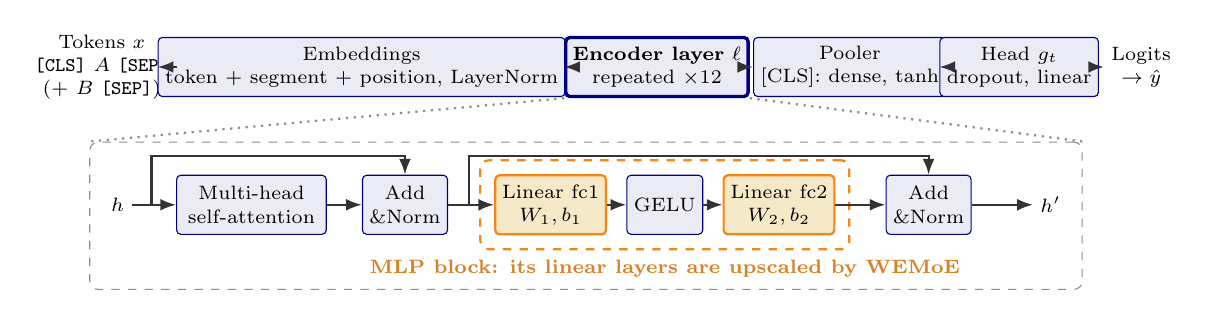
\begin{tikzpicture}[x=1cm,y=1cm]
  \tikzset{every node/.append style={font=\figfont}}
  \node[plain] (x) at (.35,0) {Tokens $x$\\ \texttt{[CLS]} $A$ \texttt{[SEP]}\\ (+ $B$ \texttt{[SEP]})};
  \node[frz,minimum width=2.35cm] (emb) at (3.65,0) {Embeddings\\ token + segment + position, LayerNorm};
  \node[frz,minimum width=2.3cm,very thick] (enc) at (7.4,0) {\textbf{Encoder layer} $\ell$\\ repeated $\times 12$};
  \node[frz,minimum width=1.75cm] (pool) at (9.85,0) {Pooler\\ {[CLS]}: dense, tanh};
  \node[frz,minimum width=1.6cm] (head) at (12.0,0) {Head $g_t$\\ dropout, linear};
  \node[plain] (out) at (13.55,0) {Logits\\ $\to\hat y$};
  \foreach \a/\b in {x/emb,emb/enc,enc/pool,pool/head,head/out} \draw[flow] (\a) -- (\b);
  \node[plain] (in) at (.55,-1.75) {$h$};
  \node[frz,minimum width=1.9cm] (att) at (2.25,-1.75) {Multi-head\\ self-attention};
  \node[frz,minimum width=.95cm] (an1) at (4.2,-1.75) {Add\\ \&Norm};
  \node[mix,minimum width=1.2cm] (fc1) at (6.05,-1.75) {Linear fc1\\ $W_1,b_1$};
  \node[frz,minimum width=.85cm] (act) at (7.5,-1.75) {GELU};
  \node[mix,minimum width=1.2cm] (fc2) at (8.95,-1.75) {Linear fc2\\ $W_2,b_2$};
  \node[frz,minimum width=.95cm] (an2) at (10.85,-1.75) {Add\\ \&Norm};
  \node[plain] (outh) at (12.4,-1.75) {$h'$};
  \foreach \a/\b in {in/att,att/an1,an1/fc1,fc1/act,act/fc2,fc2/an2,an2/outh} \draw[flow] (\a) -- (\b);
  \coordinate (r1) at ($(in.east)!.45!(att.west)$);
  \coordinate (r2) at ($(an1.east)!.45!(fc1.west)$);
  \draw[flow] (r1) -- ++(0,.62) -| (an1.north);
  \draw[flow] (r2) -- ++(0,.62) -| (an2.north);
  \begin{scope}[on background layer]
    \node[group,draw=BurntOrange,thick,fit=(fc1)(act)(fc2)] (mlp) {};
    \coordinate (ltop) at ($(r1)+(0,.62)$);
    \coordinate (lbot) at ($(mlp.south)+(0,-.32)$);
    \node[group,inner sep=5pt,fit=(in)(outh)(att)(an2)(ltop)(lbot)] (lay) {};
  \end{scope}
  \draw[black!45,dotted,thick] (enc.south west) -- (lay.north west);
  \draw[black!45,dotted,thick] (enc.south east) -- (lay.north east);
  \node[font=\figfont\bfseries,text=BurntOrange!85!black,anchor=north] at (mlp.south) {MLP block: its linear layers are upscaled by WEMoE};
\end{tikzpicture}
}
  \caption{BERT encoder as used in this study, from the input tokens to the logits (top), with one encoder layer enlarged (bottom). Dropout layers are not drawn.}
  \label{fig:bert}
\end{figure}

\section[WEMoE Architecture: Static and Input-Conditioned Merging]{WEMoE Architecture: Static and\\ Input-Conditioned Merging}

WEMoE splits the parameters into two groups. In the design of Tang et al.~\cite{tang2024wemoe}, shown in Figure~\ref{fig:overview}, attention and layer normalisation are merged statically, and each MLP is ``upscaled'' to a Weight-Ensembling MoE module, meaning that its weights become input-conditioned. Their vision Transformers normalise before each sub-layer. BERT normalises after it, so Figure~\ref{fig:arch} shows the same principle as implemented on BERT. Here the static group is every weight of the encoder outside the upscaled layers, including embeddings and pooler. Table~\ref{tab:components} lists the components, where $W_0^{\ell}$ and $\tau_i^{\ell}$ are the parts of $\theta_0$ and $\tau_i$ that belong to the MLP of layer $\ell$, $\lambda$ is the scaling factor of Section~\ref{sec:ta} and $r^{\ell}$ is the router of Section~\ref{sec:router}. The router sees only token states and does not receive the task identifier, which selects the head alone.

\begin{figure}[htbp]
  \centering
  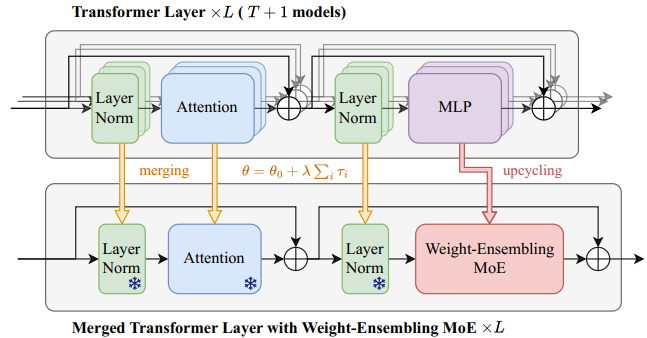
\includegraphics[width=.38\linewidth]{arch_wemoe_overview.png}
  \caption{Original WEMoE design on a pre-norm vision Transformer, from Tang et al.~\cite{tang2024wemoe}. Top: the fine-tuned and pre-trained models. Bottom: the merged layer. Frozen parts carry a snowflake mark.}
  \label{fig:overview}
\end{figure}

\begin{figure}[htbp]
  \centering
  \resizebox{.76\linewidth}{!}{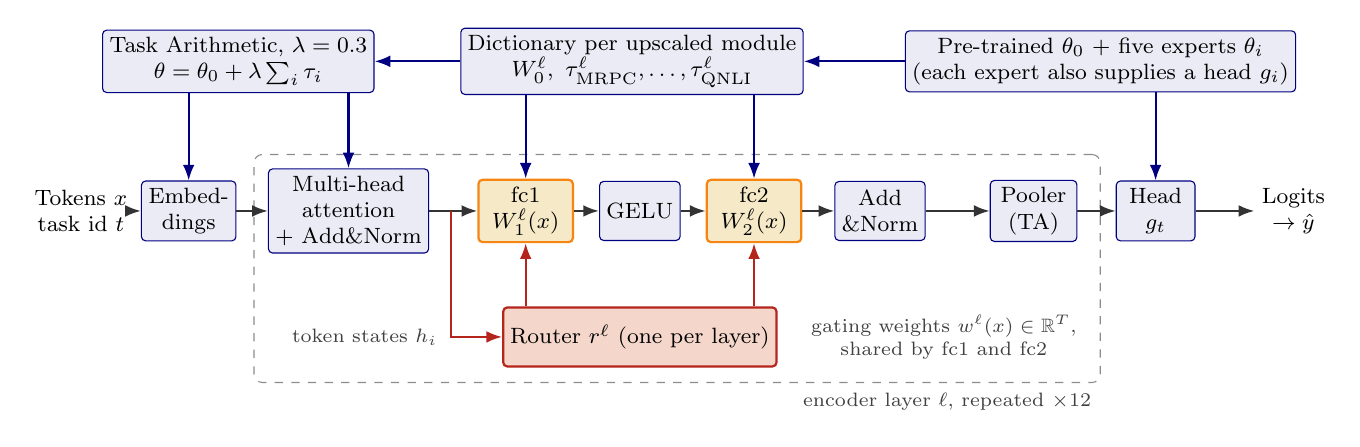
\begin{tikzpicture}[x=1cm,y=1cm]
  \node[plain] (in) at (.35,0) {Tokens $x$\\task id $t$};
  \node[frz,minimum width=1.2cm] (emb) at (1.72,0) {Embed-\\dings};
  \node[frz,minimum width=1.7cm] (att) at (3.75,0) {Multi-head\\attention\\+ Add\&Norm};
  \node[mix,minimum width=1.2cm] (fc1) at (6.0,0) {fc1\\$W^{\ell}_1(x)$};
  \node[frz,minimum width=.9cm] (act) at (7.45,0) {GELU};
  \node[mix,minimum width=1.2cm] (fc2) at (8.9,0) {fc2\\$W^{\ell}_2(x)$};
  \node[frz,minimum width=1.1cm] (nrm) at (10.5,0) {Add\\\&Norm};
  \node[frz,minimum width=1.1cm] (pool) at (12.45,0) {Pooler\\(TA)};
  \node[frz,minimum width=1.0cm] (head) at (14.0,0) {Head\\$g_t$};
  \node[plain] (out) at (15.75,0) {Logits\\$\to\hat y$};
  \foreach \a/\b in {in/emb,emb/att,att/fc1,fc1/act,act/fc2,fc2/nrm,nrm/pool,pool/head,head/out}
    \draw[flow] (\a) -- (\b);
  \node[frz,minimum width=3.4cm] (ta) at (2.35,1.9) {Task Arithmetic, $\lambda=0.3$\\$\theta=\theta_0+\lambda\sum_i\tau_i$};
  \node[frz,minimum width=4.2cm] (dict) at (7.35,1.9) {Dictionary per upscaled module\\$W_0^{\ell},\ \tau^{\ell}_{\mathrm{MRPC}},\dots,\tau^{\ell}_{\mathrm{QNLI}}$};
  \node[frz,minimum width=4.6cm] (src) at (13.3,1.9) {Pre-trained $\theta_0$ + five experts $\theta_i$\\(each expert also supplies a head $g_i$)};
  \draw[dict] (ta.south -| emb) -- (emb);
  \draw[dict] (ta.south -| att) -- (att);
  \draw[dict] (dict.south -| fc1) -- (fc1);
  \draw[dict] (dict.south -| fc2) -- (fc2);
  \draw[dict] (src.west) -- (dict.east);
  \draw[dict] (dict.west) -- (ta.east);
  \draw[dict] (src.south -| head) -- (head);
  \node[trn,minimum width=3.2cm] (rt) at (7.45,-1.6) {Router $r^{\ell}$ (one per layer)};
  \coordinate (tap) at ($(att.east)!.45!(fc1.west)$);
  \draw[gate] (tap) |- (rt.west);
  \node[note,anchor=east] at ($(tap |- rt.west)+(-.05,0)$) {token states $h_i$};
  \draw[gate] (rt.north -| fc1) -- (fc1.south);
  \draw[gate] (rt.north -| fc2) -- (fc2.south);
  \node[note,anchor=west] (gw) at (9.5,-1.6) {gating weights $w^{\ell}(x)\in\mathbb{R}^{T}$,\\shared by fc1 and fc2};
  \begin{scope}[on background layer]
    \node[group,fit=(att)(nrm)(rt)(gw)] (g) {};
  \end{scope}
  \node[note,anchor=north east] at (g.south east) {encoder layer $\ell$, repeated $\times 12$};
\end{tikzpicture}
}\\[2pt]
  \figlegend
  \caption{Merged WEMoE model as implemented. In the full scope both fc1 and fc2 are input-conditioned. In the intermediate-only scope fc2 is static and uses Task Arithmetic.}
  \label{fig:arch}
\end{figure}

\begin{table}[htbp]
  \centering\tablestyle
  \caption{Components of the merged model in the default full-MLP variant.}
  \label{tab:components}
  \begin{tabularx}{\linewidth}{l X c}
    \toprule
    Component & Origin & During FSFT\\
    \midrule
    Embeddings, attention, layer norm, pooler & Task Arithmetic with $\lambda$ chosen on dev & Frozen\\
    MLP base weights $W_0^{\ell}$ & Pre-trained model & Frozen\\
    MLP task vectors $\tau_i^{\ell}$ & Experts minus pre-trained model & Frozen\\
    Classification heads $g_t$ & One from each expert & Frozen\\
    Routers $r^{\ell}$ & New, one per encoder layer & \textbf{Trained}\\
    \bottomrule
  \end{tabularx}
\end{table}

The split sets the storage cost. A static part is stored once. Each upscaled layer must keep its pre-trained weights and one task vector per expert, which is $T+1$ copies of that layer, and the routers add their own parameters $\phi$:
\begin{equation}
|\theta_{\mathrm{static}}|+(T+1)\,|\theta_{\mathrm{MLP}}|+|\phi|+|\mathrm{heads}|,
\label{eq:storage}
\end{equation}
where $\theta_{\mathrm{MLP}}$ denotes the upscaled layers. We evaluate two scopes: \emph{full}, which upscales fc1 and fc2, and \emph{intermediate-only}, which upscales fc1 alone. The task vectors account for most of the stored parameters of the full scope (Table~\ref{tab:storage}), so the saving depends strongly on this choice. Tang et al.\ base the choice of the MLP on their observation for CLIP-ViT models that attention weights stay closer in direction to the pre-trained model than MLP weights do. We did not repeat that measurement on BERT, so the choice is inherited and not independently justified here.

\section{Task Arithmetic and Task Vectors}
\label{sec:ta}

A task vector (Equation~\ref{eq:task-vector}) records what fine-tuning changed for a task. Task Arithmetic~\cite{ilharco2023task} adds the vectors back to the base with one scaling factor $\lambda$:
\begin{equation}
\theta=\theta_0+\lambda\sum_{i=1}^{T}\tau_i .
\label{eq:ta}
\end{equation}
Simple Averaging is the special case $\lambda=1/T$, which equals the mean of the expert weights. A small $\lambda$ stays near the pre-trained model, and a large one applies the updates more strongly, including any conflicts among them. We select $\lambda$ by grid search on the mean development score (Section~\ref{sec:merging}). The method is simple and adds no parameters, but its result is the same for every input.

\section{Router and Input-Conditioned MLP}
\label{sec:router}

Each encoder layer has its own router $r^{\ell}$ (Figure~\ref{fig:router}). Its input is the sequence of token states $h^{\ell}_j\in\mathbb{R}^{d}$ that leave the first Add\&Norm of the layer. The router has two linear layers with a ReLU and is applied to every token:
\begin{equation}
r^{\ell}(h)=A^{\ell}_2\,\mathrm{ReLU}\big(A^{\ell}_1h+c^{\ell}_1\big)+c^{\ell}_2,
\label{eq:router}
\end{equation}
with $A^{\ell}_1\in\mathbb{R}^{d\times d}$ and $A^{\ell}_2\in\mathbb{R}^{T\times d}$. The twelve routers hold $12\,(d^2+d+Td+T)=7{,}133{,}244$ trainable parameters. Token outputs are averaged over non-padding positions, using the attention mask $m_j\in\{0,1\}$, to give one vector per input, so that padding does not affect routing:
\begin{equation}
w^{\ell}(x)=\frac{\sum_j m_j\,r^{\ell}(h^{\ell}_j)}{\sum_j m_j}\in\mathbb{R}^{T}.
\label{eq:gating}
\end{equation}
For an input $x$, each upscaled linear layer is rebuilt from its pre-trained weights and its part of the task vectors, and its bias is rebuilt in the same way:
\begin{equation}
W^{\ell}(x)=W_0^{\ell}+\sum_{i=1}^{T}w_i^{\ell}(x)\,\tau_i^{\ell},\qquad
b^{\ell}(x)=b_0^{\ell}+\sum_{i=1}^{T}w_i^{\ell}(x)\,\tau_i^{\ell,b}.
\label{eq:we}
\end{equation}
Both linear layers of a block share the same $w^{\ell}(x)$. The prediction uses the head $g_t$ of the known task, where $\bar\theta$ denotes the statically merged weights:
\begin{equation}
p(y\mid x,t)=\mathrm{softmax}\Big(g_t\big(\mathrm{pool}(\mathrm{BERT}(x;\bar\theta,\{W^{\ell}(x)\}))\big)\Big),\quad
\hat y=\arg\max_{y}\,p(y\mid x,t).
\label{eq:prediction}
\end{equation}

\begin{figure}[htbp]
  \centering
  \begin{minipage}[c]{.25\linewidth}\centering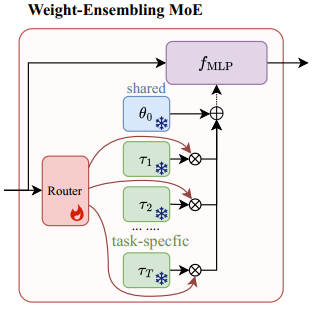
\includegraphics[width=\linewidth]{arch_wemoe_module.png}\end{minipage}\hfill
  \begin{minipage}[c]{.72\linewidth}\centering\resizebox{\linewidth}{!}{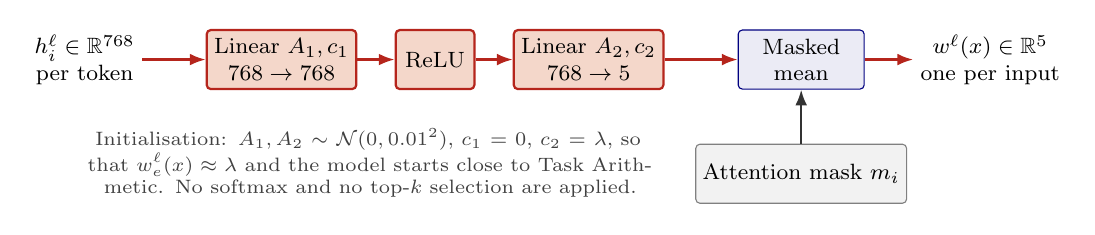
\begin{tikzpicture}[x=1cm,y=1cm]
  \node[plain] (h) at (0,0) {$h^{\ell}_i\in\mathbb{R}^{768}$\\per token};
  \node[trn,minimum width=1.9cm] (a1) at (2.5,0) {Linear $A_1,c_1$\\$768\to768$};
  \node[trn,minimum width=1.0cm] (re) at (4.45,0) {ReLU};
  \node[trn,minimum width=1.9cm] (a2) at (6.4,0) {Linear $A_2,c_2$\\$768\to5$};
  \node[frz,minimum width=1.6cm] (mm) at (9.1,0) {Masked\\mean};
  \node[plain] (w) at (11.5,0) {$w^{\ell}(x)\in\mathbb{R}^{5}$\\one per input};
  \foreach \a/\b in {h/a1,a1/re,re/a2,a2/mm,mm/w} \draw[gate] (\a) -- (\b);
  \node[dat,minimum width=2.1cm] (m) at (9.1,-1.45) {Attention mask $m_i$};
  \draw[flow] (m) -- (mm);
  \node[note,text width=7.2cm,anchor=north] at (3.6,-.75) {Initialisation: $A_1,A_2\sim\mathcal{N}(0,0.01^2)$, $c_1=0$, $c_2=\lambda$, so that $w_e^{\ell}(x)\approx\lambda$ and the model starts close to Task Arithmetic. No softmax and no top-$k$ selection are applied.};
\end{tikzpicture}
}\end{minipage}
  \caption{Left: the WEMoE module of Tang et al.~\cite{tang2024wemoe}. Right: router of layer $\ell$ as implemented, applied per token and averaged over non-padding tokens.}
  \label{fig:router}
\end{figure}

The router's values are \emph{unnormalised}. With no softmax and no top-$k$ selection, a value can exceed 1 or be negative, so a router can amplify or subtract a task vector, and the combination is neither convex nor sparse. Linear weights are initialised from $\mathcal{N}(0,0.01^2)$ with $c^{\ell}_1=0$ and $c^{\ell}_2=\lambda$, so $w^{\ell}_i(x)\approx\lambda$ at the start and the model begins close to Task Arithmetic. Unit tests on small random models confirm that constant routing equals Task Arithmetic, that padding does not affect routing and that only the routers receive gradients.

\section{Few-Shot Fine-Tuning (FSFT) Objective}
\label{sec:fsft}

The routers are trained with Few-Shot Fine-Tuning: cross-entropy on a small labelled set, summed over the tasks. For each task, $k$ examples $D_t^{(k)}$ are drawn from a reserved pool, and for a fixed seed a smaller $k$ gives a subset of a larger one. At each step, one mini-batch $B_t$ is drawn per task, and the objective is
\begin{equation}
\min_{\phi}\ \sum_{t=1}^{T}\ \frac{1}{|B_t|}\sum_{(x,y)\in B_t}-\log p_{\phi}(y\mid x,t),
\qquad B_t\subset D_t^{(k)},\ \ |D_t^{(k)}|=k ,
\label{eq:fsft}
\end{equation}
where $p_\phi$ is the distribution of Equation~\eqref{eq:prediction}. Everything except $\phi$ stays frozen, and dropout is disabled. The mean development score is evaluated before training and every 50 steps, and the router state of the best step is restored at the end. A run whose best step is 0 therefore reports the untrained router.

Table~\ref{tab:comparison} separates the original method from this study. The largest difference is the objective. Tang et al.\ minimise prediction entropy on unlabelled test data, which is test-time adaptation, and this objective is not used here. FSFT instead uses labelled training examples and never touches the reporting split. The results of the two studies are therefore not directly comparable.

\begin{table}[htbp]
  \centering\tablestyle
  \caption{The original WEMoE study of Tang et al.~\cite{tang2024wemoe} and this study.}
  \label{tab:comparison}
  \begin{tabularx}{\linewidth}{>{\bfseries\raggedright\arraybackslash}p{2.9cm} *{2}{>{\raggedright\arraybackslash}X}}
    \toprule
    Aspect & Tang et al. & This study\\
    \midrule
    Backbone, tasks & CLIP-ViT vision models; eight image classification tasks & BERT-base; five binary GLUE tasks\\
    Router training & Test-time adaptation: entropy on unlabelled test data & FSFT: cross-entropy on $k$ labelled examples per task\\
    Routing input & Mean over tokens & Mean over non-padding tokens\\
    Upscaled modules & Transformer MLPs & Full MLP; intermediate-only as an ablation\\
    \bottomrule
  \end{tabularx}
\end{table}


\chapter{Experimental Methodology}
\label{ch:method}
\section{The Five Binary GLUE Tasks and Their Datasets}

The experiments use five binary tasks of the General Language Understanding Evaluation benchmark (GLUE)~\cite{wang2019glue}, loaded through the Hugging Face Datasets library~\cite{lhoest2021datasets} and listed in Table~\ref{tab:data}: MRPC~\cite{dolan2005mrpc}, RTE~\cite{dagan2006rte}, CoLA~\cite{warstadt2019cola}, SST-2~\cite{socher2013sst} and QNLI, which is derived from SQuAD~\cite{rajpurkar2016squad}. CoLA and SST-2 take a single sentence, while MRPC, RTE and QNLI take a pair. Inputs are tokenised and truncated to 128 tokens. The tasks differ widely in size, as Table~\ref{tab:split} shows, and in how much a constant prediction scores, as the last column of Table~\ref{tab:data} shows.

\begin{table}[htbp]
  \centering\tablestyle
  \caption{The five GLUE tasks. ``Maj.\ \%'' is the validation accuracy of always predicting the most frequent label.}
  \label{tab:data}
  \setlength{\tabcolsep}{3.5pt}\begin{tabularx}{\linewidth}{l X l l l r}
    \toprule
    Task & Decides whether\ldots & Input fields & Labels & Metric & Maj.\ \%\\
    \midrule
    MRPC & two sentences are paraphrases & sentence1, sentence2 & not\_equivalent / equivalent & acc + F1 & 68.4\\
    RTE & a sentence entails another & sentence1, sentence2 & entailment / not\_entailment & accuracy & 52.7\\
    CoLA & a sentence is grammatical & sentence & unacceptable / acceptable & MCC & 69.1\\
    SST-2 & a sentence is positive or negative & sentence & negative / positive & accuracy & 50.9\\
    QNLI & a sentence answers a question & question, sentence & entailment / not\_entailment & accuracy & 50.5\\
    \bottomrule
  \end{tabularx}
\end{table}

\section{Data Splits and Experimental Protocol}
\label{sec:protocol}

The official training split of each task is permuted once with seed 42 and divided into three disjoint parts (Table~\ref{tab:split}). Four kinds of data therefore have distinct roles:

\begin{itemize}
  \item \textbf{Expert training data} is everything left after the two reservations below. Only the experts train on it.
  \item \textbf{The few-shot pool} holds 256 labelled examples per task, and $k$ of them train the routers. The experts never see it.
  \item \textbf{The development split} (dev) is 10\% of the official training split, with at most 1,000 examples. It makes every choice: expert epoch, $\lambda$ and FSFT step.
  \item \textbf{The official validation split} is used for reported scores only.
\end{itemize}

GLUE test splits are not used. Their labels are hidden in the dataset for four of the tasks, and the MRPC test labels were also left unused. This protocol prevents the main forms of leakage, at a cost: RTE, the smallest task, keeps only 1,985 of its 2,490 training pairs for its expert.

\begin{table}[htbp]
  \centering\tablestyle
  \caption{Data splits per task. The last row gives the use of each split.}
  \label{tab:split}
  \begin{tabular}{l r r r r r}
    \toprule
    Task & Official train & Few-shot pool & Dev & Expert train & Official validation\\
    \midrule
    MRPC & 3,668 & 256 & 367 & 3,045 & 408\\
    RTE & 2,490 & 256 & 249 & 1,985 & 277\\
    CoLA & 8,551 & 256 & 855 & 7,440 & 1,043\\
    SST-2 & 67,349 & 256 & 1,000 & 66,093 & 872\\
    QNLI & 104,743 & 256 & 1,000 & 103,487 & 5,463\\
    \midrule
    \textbf{Used for} & & \textbf{FSFT} & \textbf{Selection} & \textbf{Experts} & \textbf{Reporting}\\
    \bottomrule
  \end{tabular}
\end{table}

\section{Training the Five Task-Specific Experts}

Each expert fine-tunes all layers of \texttt{bert-base-uncased} and a new two-class head with cross-entropy on its expert-training data. All five use one recipe, shown in the first column of Table~\ref{tab:config}, with no per-task tuning, and the best of three epochs is chosen on dev by task score. AdamW~\cite{loshchilov2019adamw} applies weight decay only to parameters with at least two dimensions.

\begin{table}[htbp]
  \centering\tablestyle
  \caption{Training configuration of the two optimisation stages.}
  \label{tab:config}
  \begin{tabularx}{\linewidth}{>{\bfseries}l *{2}{>{\raggedright\arraybackslash}X}}
    \toprule
    Setting & Task-specific experts & FSFT (routers)\\
    \midrule
    Trainable parameters & All of BERT and the head (109.5M per expert) & Routers only (7.1M); 60 in the input-independent variant\\
    Optimiser & AdamW; weight decay 0.01 & AdamW; no weight decay\\
    Learning rate & $2\times10^{-5}$ & $10^{-4}$; $10^{-3}$ in the input-independent variant\\
    Schedule & Linear, 10\% warm-up & Linear, 10\% warm-up\\
    Batch size, duration & 32; 3 epochs & 16 per task; 500 steps\\
    Gradient clipping & Norm 1.0 & None\\
    Selection on dev & Best epoch by task score & Best step by mean score, every 50 steps\\
    \bottomrule
  \end{tabularx}
\end{table}

\section{Merging the Experts and Training the Router with Few-Shot Data}
\label{sec:merging}

Task Arithmetic selects $\lambda$ from $\{0.1,0.2,\dots,1.0\}$ by the mean dev score (Table~\ref{tab:lambda}). The score peaks at $\lambda=0.3$, and this value initialises the merged models. Dev can mislead for merged models on SST-2: at $\lambda=0.3$, Task Arithmetic scores 83.7 on dev but 69.8 on validation. The two splits differ in kind, since SST-2 training texts average 9.4 words and validation texts 19.5. Selecting on dev remains the correct procedure, but its SST-2 scores overstate merged-model quality.

\begin{table}[htbp]
  \centering\tablestyle
  \caption{Development scores of Task Arithmetic over the $\lambda$ grid ($\times100$).}
  \label{tab:lambda}
  \begin{tabular}{l c c c c c c c c c c}
    \toprule
    $\lambda$ & 0.1 & 0.2 & \textbf{0.3} & 0.4 & 0.5 & 0.6 & 0.7 & 0.8 & 0.9 & 1.0\\
    \midrule
    Mean dev score & 52.0 & 57.4 & \textbf{62.8} & 60.7 & 58.6 & 58.0 & 57.5 & 57.3 & 57.4 & 57.1\\
    SST-2 dev score & 62.4 & 73.3 & \textbf{83.7} & 89.8 & 91.7 & 92.3 & 93.0 & 93.2 & 92.9 & 92.5\\
    \bottomrule
  \end{tabular}
\end{table}

Fifteen FSFT runs were performed, three seeds for each of five configurations. The main model is \emph{full-MLP} WEMoE with $k\in\{16,64,256\}$. Two \emph{ablations}, which change one component and keep the rest fixed, use $k=256$. The \emph{intermediate-only} variant upscales fc1 alone, and fc2 uses Task Arithmetic. The \emph{input-independent} variant has no router: it learns one coefficient per expert per layer, the same for every input, for 60 numbers in total. It starts exactly at Task Arithmetic and tests whether routing on the input is needed. Its learning rate is higher because it has so few parameters.

\section{Evaluation Metrics, Baselines, Seeds and Reproducibility}
\label{sec:metrics}

\paragraph{Metrics.} Scores are multiplied by 100. The \emph{task score} $S_t$ follows GLUE conventions: the mean of accuracy and F1 for MRPC, the Matthews Correlation Coefficient (MCC)~\cite{matthews1975mcc} for CoLA, and accuracy for the others. MCC is a correlation between predictions and labels, and a constant prediction scores 0. The \emph{average score} is the unweighted mean of the five task scores, and the \emph{normalised score} is the mean of $S_t(m)/S_t(\mathrm{expert})$ for a model $m$. A constant prediction already scores about 75 on MRPC and about 50 on the accuracy tasks, so the normalised score flatters weak models. The \emph{gain over majority} corrects for this, with 0 for a constant guess and 100 for the expert:
\begin{equation}
\mathrm{Gain}(m)=\frac{100}{T}\sum_{t=1}^{T}\frac{S_t(m)-S_t(\mathrm{majority})}{S_t(\mathrm{expert})-S_t(\mathrm{majority})}.
\label{eq:gain}
\end{equation}

\paragraph{Baselines.} The \emph{majority class} always predicts the most frequent validation label, which is the score of a model collapsed to a constant prediction. \emph{Simple Averaging} is Task Arithmetic with $\lambda=1/5$. \emph{Task Arithmetic} uses the selected $\lambda=0.3$. \emph{WEMoE init} is the merged model before router training. The five experts are the upper reference point.

\paragraph{Seeds and reproducibility.} The data split and the experts use seed 42. FSFT uses seeds 0, 1 and 2, where a seed sets the router initialisation and the few-shot sample, while the experts and the data split stay fixed. Runs used Google Colab with one NVIDIA Tesla T4 GPU and mixed precision, with PyTorch 2.11.0, Datasets 4.8.5 and scikit-learn 1.6.1. The recorded Transformers~\cite{wolf2020transformers} version is 5.20.2 for the experts and most FSFT runs, and 5.22.0 for the baseline evaluation and the input-independent runs.


\chapter{Results}
\label{ch:results}
All scores come from the official validation splits. WEMoE rows give the mean and standard deviation over seeds 0, 1 and 2.

\section{Results by Task}

Table~\ref{tab:per-task} and Figure~\ref{fig:per-task} give the scores per task, and Table~\ref{tab:gain} places each merged model between the majority class and the expert. The experts themselves are not equally strong. SST-2 and QNLI, with the most training data, score above 90. RTE scores only 63.2, and its dev score was still rising at the last epoch (49.0, 65.5, 65.9). Expert training took 43 minutes in total: 0.8, 0.7, 1.1, 11.0 and 29.8 minutes for MRPC, RTE, CoLA, SST-2 and QNLI, with best epochs 2, 3, 3, 2 and 3.

\begin{table}[htbp]
  \centering\tablestyle
  \caption{Per-task scores ($\times100$). Bold marks the WEMoE $k=256$ results that fall below the majority class.}
  \label{tab:per-task}
  \setlength{\tabcolsep}{3pt}\begin{tabular}{l c c c c c}
    \toprule
    Model & MRPC (Acc/F1) & RTE (Acc) & CoLA (MCC) & SST-2 (Acc) & QNLI (Acc)\\
    \midrule
    Majority class & 68.4 / 81.2 & 52.7 & 0.0 & 50.9 & 50.5\\
    Simple Averaging & 68.4 / 81.2 & 46.9 & 23.3 & 55.4 & 65.9\\
    Task Arithmetic & 68.6 / 81.3 & 47.3 & 16.9 & 69.8 & 77.9\\
    Input-independent, $k$=256 & 68.4 / 81.2 & 47.3 & 20.2$\pm$0.0 & 70.9$\pm$0.1 & 78.6$\pm$0.0\\
    WEMoE full, $k$=16 & 68.7$\pm$2.3 / 80.6$\pm$2.2 & 48.0$\pm$1.0 & 27.6$\pm$14.1 & 79.6$\pm$8.1 & 74.0$\pm$6.5\\
    WEMoE full, $k$=64 & 71.6$\pm$4.4 / 80.9$\pm$4.3 & 54.0$\pm$3.4 & 20.5$\pm$17.8 & 89.0$\pm$0.6 & 83.1$\pm$2.4\\
    WEMoE full, $k$=256 & 76.3$\pm$4.5 / 83.9$\pm$2.8 & \textbf{52.0$\pm$4.4} & 42.6$\pm$0.9 & 88.0$\pm$0.5 & 86.7$\pm$0.7\\
    WEMoE intermediate, $k$=256 & \textbf{66.5$\pm$0.7 / 76.6$\pm$1.0} & 59.0$\pm$0.9 & 41.7$\pm$0.9 & 86.7$\pm$0.2 & 86.5$\pm$0.2\\
    Single-task experts & 82.1 / 88.1 & 63.2 & 59.1 & 92.2 & 91.2\\
    \bottomrule
  \end{tabular}
\end{table}

\begin{figure}[htbp]
  \centering
  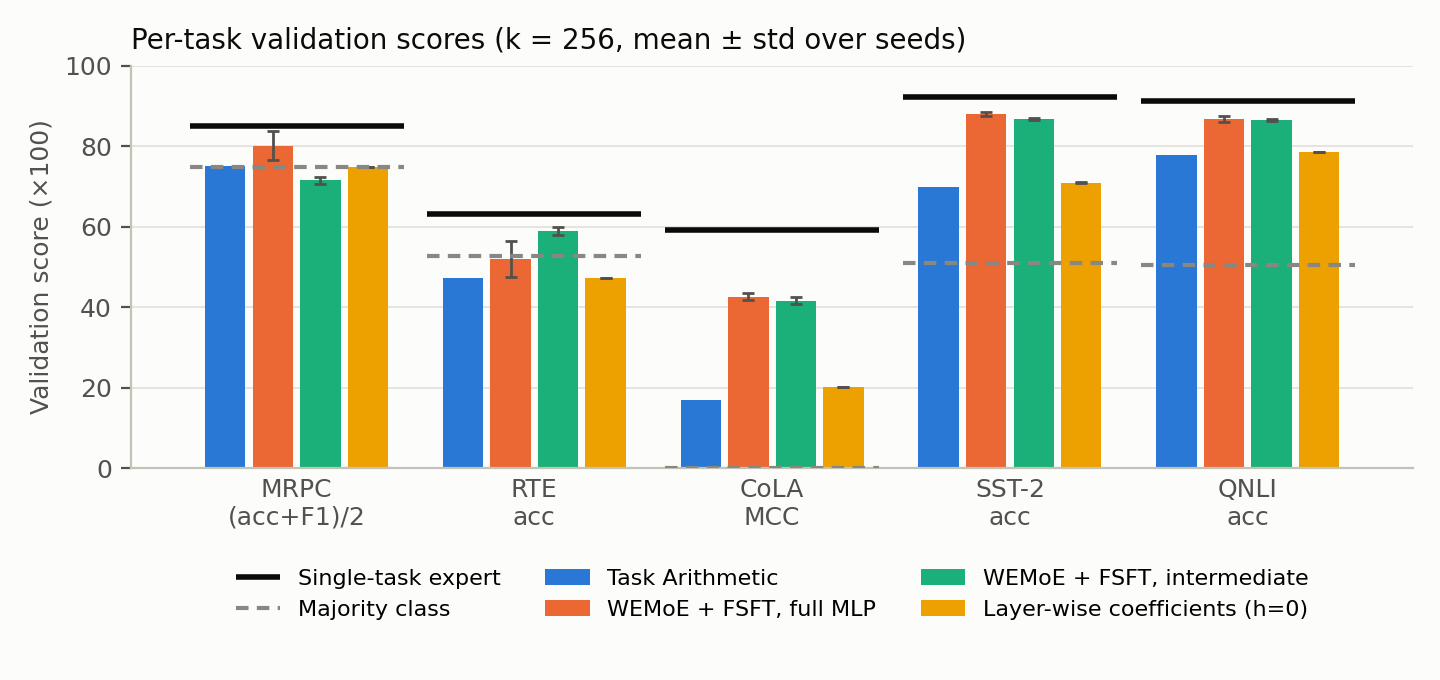
\includegraphics[width=.85\linewidth]{per_task.png}
  \caption{Task scores of the merged models between the majority class (dashed tick) and the experts (solid tick). WEMoE values use $k=256$; bars are means over three seeds and error bars their standard deviation. The yellow bars are the input-independent ablation (layer-wise coefficients, $h=0$).}
  \label{fig:per-task}
\end{figure}

\begin{table}[htbp]
  \centering\tablestyle
  \caption{Gain over majority per task, in percent, computed from the seed means.}
  \label{tab:gain}
  \begin{tabular}{l r r r r r r}
    \toprule
    Model & MRPC & RTE & CoLA & SST-2 & QNLI & Mean\\
    \midrule
    Task Arithmetic & 1.8 & $-51.7$ & 28.6 & 45.8 & 67.3 & 18.4\\
    Input-independent, $k=256$ & 0.0 & $-51.7$ & 34.2 & 48.5 & 68.9 & 20.0\\
    WEMoE full, $k=256$ & 51.5 & $-6.9$ & 72.2 & 89.7 & 88.9 & 59.1\\
    WEMoE intermediate, $k=256$ & $-31.6$ & 59.8 & 70.5 & 86.8 & 88.5 & 54.8\\
    \bottomrule
  \end{tabular}
\end{table}

The average improvement does not apply uniformly. On SST-2 and QNLI, the trained routers recover close to 90\% of the gain, and on CoLA about 70\%, against 45.8, 67.3 and 28.6 for Task Arithmetic. Static merging is close to a constant prediction on the two smallest tasks. Its RTE accuracy of 47.3 equals 131/277, the share of the \emph{minority} class, which is consistent with one label for every example, and its MRPC scores barely differ from the majority class. WEMoE does not fully repair this. The full-MLP model recovers about half of the gain on MRPC but does not reliably beat the majority class on RTE: its three seeds give 49.5, 57.0 and 49.5, against 52.7. The intermediate-only model recovers 59.8\% on RTE but falls below the majority class on MRPC. No merged model matches an expert on any task.

\section{Comparison with Relevant Baselines}

Table~\ref{tab:main} gives the aggregate comparison. Task Arithmetic reaches 57.4 and recovers only 18.4\% of the gain, although its normalised score of 70.6 would suggest much more. Before training, the full-MLP model is close to it ($57.8\pm0.6$) but not identical, because the small random router weights move CoLA in particular. At $k=256$, FSFT raises the model to $69.9\pm0.1$, which is 12.5 points above Task Arithmetic and 8.3 below the experts, with a gain of $59.1\pm1.1$.

\begin{table}[htbp]
  \centering\tablestyle
  \caption{Aggregate results ($\times100$). ``Init'' is WEMoE before router training. Time covers one FSFT run on the T4, including dev evaluations.}
  \label{tab:main}
  \begin{tabular}{l c c c c r}
    \toprule
    Model & Average & Normalised & Gain & Best step of 500 & Min\\
    \midrule
    Majority class & 45.8 & 56.4 & 0.0 & -- & --\\
    Simple Averaging & 53.3 & 66.8 & 6.6 & -- & --\\
    Task Arithmetic ($\lambda=0.3$) & 57.4 & 70.6 & 18.4 & -- & --\\
    Init, full MLP & 57.8$\pm$0.6 & 71.3$\pm$1.0 & 18.7$\pm$1.5 & -- & --\\
    Init, intermediate-only & 57.5$\pm$0.4 & 70.8$\pm$0.6 & 18.1$\pm$1.2 & -- & --\\
    Input-independent, $k=256$ & 58.4$\pm$0.0 & 72.0$\pm$0.0 & 20.0$\pm$0.0 & 50, 50, 50 & 15.4\\
    WEMoE full, $k=16$ & 60.8$\pm$2.7 & 75.6$\pm$4.6 & 25.5$\pm$4.6 & 50, 0, 150 & 16.3\\
    WEMoE full, $k=64$ & 64.6$\pm$3.7 & 79.5$\pm$6.3 & 46.7$\pm$8.5 & 100, 250, 100 & 14.4\\
    \textbf{WEMoE full, $k=256$} & \textbf{69.9$\pm$0.1} & \textbf{87.8$\pm$0.5} & \textbf{59.1$\pm$1.1} & 250, 200, 200 & 16.3\\
    WEMoE intermediate, $k=256$ & 69.1$\pm$0.1 & 87.4$\pm$0.1 & 54.8$\pm$1.7 & 500, 400, 400 & 8.4\\
    Single-task experts & 78.2 & 100.0 & 100.0 & -- & --\\
    \bottomrule
  \end{tabular}
\end{table}

\paragraph{Input-independent ablation.} Coefficients fixed for all inputs barely move the score ($58.4\pm0.0$, gain 20.0). They start at the dev score of Task Arithmetic (62.8), stay between 62.4 and 63.0 throughout training, and reach their best score at step 50 on every seed. The learned coefficients lie within 0.023 of their starting value of 0.3. Over the same 500 steps, the full-MLP routers start between 62.6 and 62.9 on dev and reach best scores of 72.6, 73.0 and 72.9. Only one learning rate was tried for this variant.

\paragraph{Few-shot budget.} Figure~\ref{fig:k-sweep} shows that the average rises with $k$ and has not levelled off at 256. Small budgets vary strongly across seeds. The budget effect is also not monotonic on every task: CoLA MCC has a mean of 27.6 at $k=16$ and 20.5 at $k=64$, with runs spanning 18--44 and 9--41, and then $42.6\pm0.9$ at $k=256$. For seed 1 at $k=16$, no step beat the untrained router on dev, so that run reports WEMoE init. At $k=256$, every task has a standard deviation of at most 0.9 except MRPC and RTE, so the stable average hides seed variation on those two.

\begin{figure}[htbp]
  \centering
  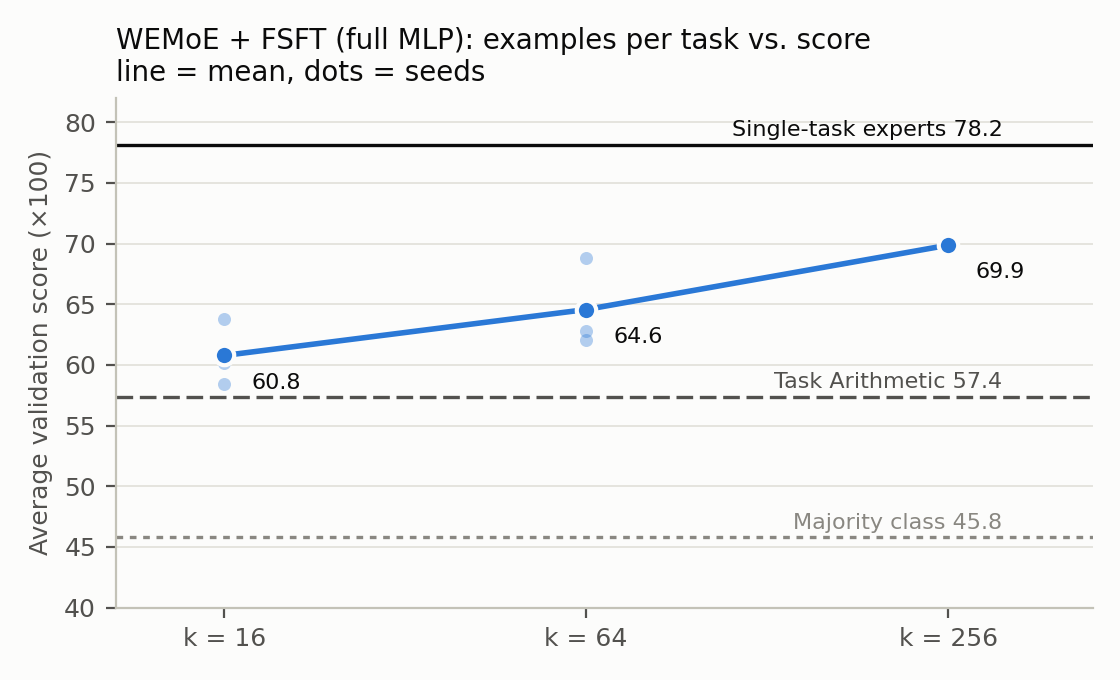
\includegraphics[width=.6\linewidth]{k_sweep.png}
  \caption{Average validation score of full-MLP WEMoE against the few-shot budget. The line shows the mean, and the dots show the seeds.}
  \label{fig:k-sweep}
\end{figure}

\section{Routing Behaviour}
\label{sec:routing}

Figure~\ref{fig:routing} shows the mean router values per layer and input task for one trained model. Many values lie far from their initial value of about $\lambda$, and both signs occur, which a convex mixture could not express. The panels look broadly alike, so much of the pattern is shared across input tasks, although they also differ in places, which shows that routing depends in part on the input. In this model, the column of the RTE expert is negative in the last two layers for every input type.

\begin{figure}[htbp]
  \centering
  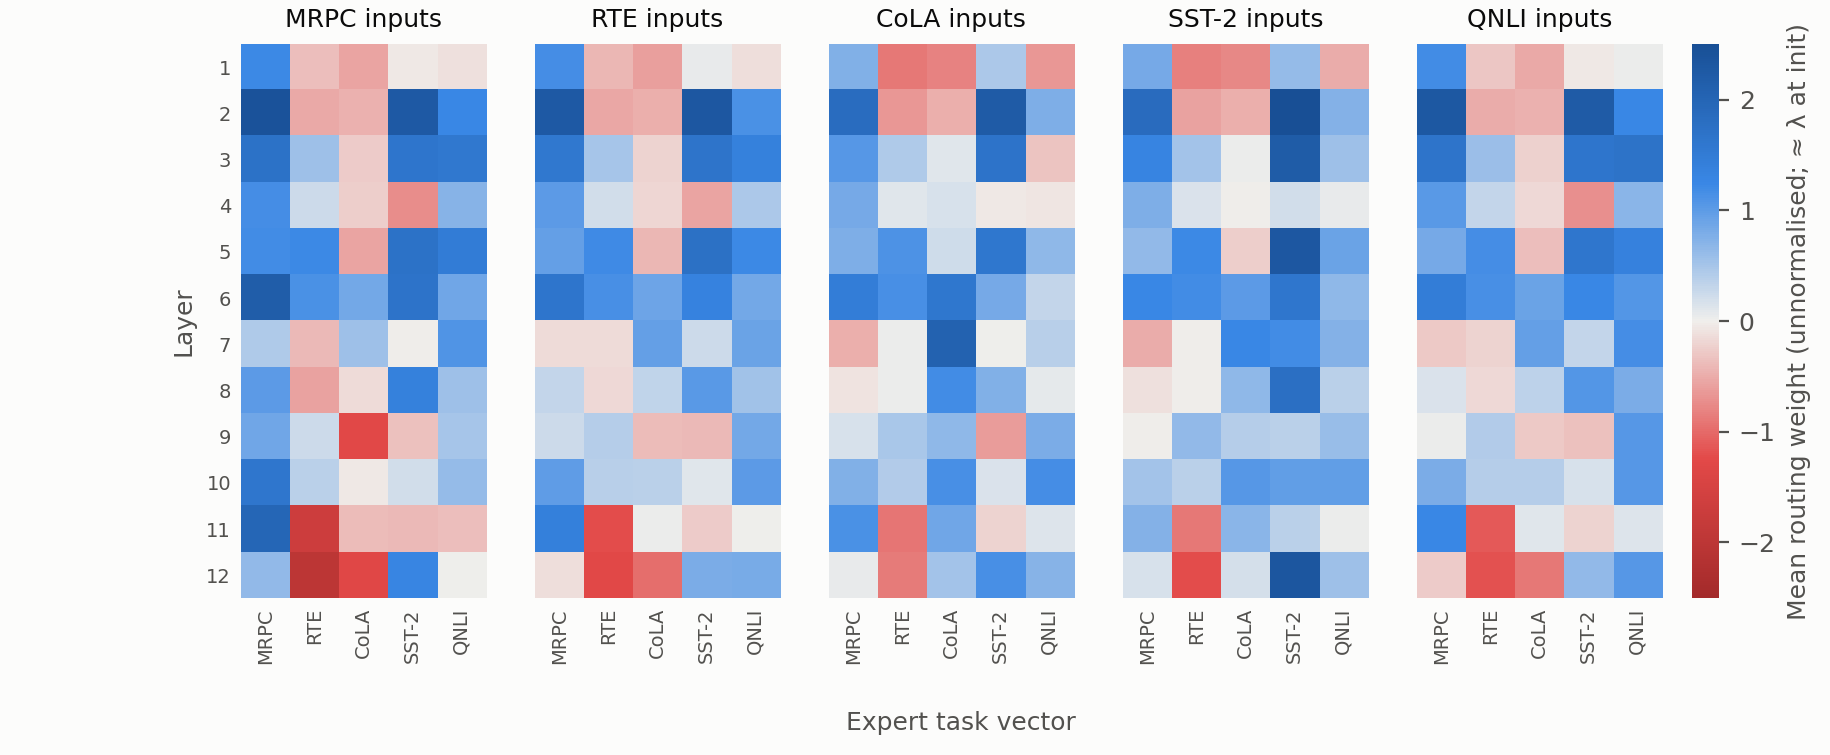
\includegraphics[width=.6\linewidth]{routing_clean.png}
  \caption{Mean router values per layer and input task (full MLP, $k=256$, seed 0). Blue adds and red subtracts a task vector.}
  \label{fig:routing}
\end{figure}

We quantified this pattern from the router values of every validation example. For seed 0, individual values range from $-3.0$ to $4.4$, and the per-layer sum of the values averaged over all examples reaches 5.8, against 1.5 at initialisation. The mean routing matrices of different input tasks correlate at 0.82 on average (0.84 for seeds 1 and 2), while the input task explains about 58\% of the routing variance (60\% for seeds 1 and 2). Table~\ref{tab:own} shows that most tasks up-weight their own expert, with RTE as the exception.

The RTE expert behaves differently across scopes, and one seed is not enough to read this difference. Its value on RTE inputs at layer 12 is negative under full-MLP upscaling on all three seeds ($-1.28$, $-0.65$, $-0.76$) and positive under intermediate-only upscaling ($2.04$, $1.16$, $1.53$). Its value averaged over layers is less stable: under intermediate-only upscaling it is 0.96, 0.27 and 0.31, while RTE accuracy stays between 58.1 and 59.9, so this average does not explain the RTE result. This evidence shows association only and does not establish why RTE fails.

\begin{table}[htbp]
  \centering\tablestyle
  \caption{Mean router value of a task's own expert, averaged over layers (full MLP, $k=256$, seed 0).}
  \label{tab:own}
  \begin{tabular}{l c c c c c}
    \toprule
    & MRPC & SST-2 & QNLI & CoLA & RTE\\
    \midrule
    On its own inputs & 1.37 & 1.37 & 0.94 & 0.61 & 0.01\\
    On other tasks' inputs & 0.77 & 0.67 & 0.56 & $-0.02$ & $-0.01$\\
    \bottomrule
  \end{tabular}
\end{table}

\section{Storage, Parameter Count and Inference Latency}
\label{sec:efficiency}

Table~\ref{tab:storage} breaks down the stored parameters, which match Equation~\eqref{eq:storage} and are measured on the built models. Task vectors dominate, at 283.3M of the 400.0M parameters of the full-MLP model.

\begin{table}[htbp]
  \centering\tablestyle
  \caption{Stored parameters (millions) by component, and total size at 32-bit precision.}
  \label{tab:storage}
  \setlength{\tabcolsep}{4pt}\begin{tabular}{l r r r r r r r r}
    \toprule
    Deployment & Static & Base MLP & Task vectors & Routers & Heads & Total & GiB & vs.\ 5 models\\
    \midrule
    5 single-task models & -- & -- & -- & -- & -- & 547.4 & 2.04 & 100.0\%\\
    Task Arithmetic & -- & -- & -- & -- & -- & 109.5 & 0.41 & 20.0\%\\
    WEMoE, full MLP & 52.8 & 56.7 & 283.3 & 7.13 & 0.008 & 400.0 & 1.49 & 73.1\%\\
    WEMoE, intermediate-only & 81.1 & 28.3 & 141.7 & 7.13 & 0.008 & 258.4 & 0.96 & 47.2\%\\
    \bottomrule
  \end{tabular}
\end{table}

Table~\ref{tab:latency} reports latency on one T4 GPU, with random token ids of length 128, mixed precision and the MRPC head, as the mean of 10 forward passes after 3 warm-up passes. The single-task row times one expert, because each input would go to its own expert by task identifier. Batch-1 figures are rough: they differed by up to 27\% between two measurement runs (24.05 ms and 18.90 ms for the intermediate-only model), while batch-32 times agreed within about 5\%. At batch size 32, the full-MLP model is about 4.5 times slower than one BERT and the intermediate-only model about 2.9 times, and the full-MLP model needs about 2.8 times the peak GPU memory.

\begin{table}[htbp]
  \centering\tablestyle
  \caption{Inference latency and peak GPU memory on one T4, from the final measurement run. $^{*}$Times one expert.}
  \label{tab:latency}
  \begin{tabular}{l c c c c}
    \toprule
    & \multicolumn{2}{c}{Batch 1} & \multicolumn{2}{c}{Batch 32}\\
    Deployment & ms/example & Peak MB & ms/example & Peak MB\\
    \midrule
    Single-task BERT$^{*}$ & 11.64 & 614 & 1.61 & 704\\
    Task Arithmetic & 12.67 & 435 & 1.63 & 519\\
    WEMoE, full MLP & 27.83 & 1615 & 7.31 & 1987\\
    WEMoE, intermediate-only & 18.90 & 1061 & 4.69 & 1387\\
    \bottomrule
  \end{tabular}
\end{table}


\chapter{Trade-offs and Discussion}
\label{ch:discussion}
\section{What the Results Demonstrate}

The measurements show three things in this setting. Static merging performs close to a constant prediction on the two smallest tasks. Routers trained on 256 examples per task raise the average score by 12.5 points and the gain over majority from 18.4 to 59.1. Fixed coefficients trained on the same data improve the average by only 1 point.

Our interpretation is that input-dependent routing accounts for most of the improvement over Task Arithmetic. This goes beyond the direct measurement, because the two variants also differ in capacity (7.1M against 60 parameters) and in learning rate, and only one learning rate was tried for the ablation, although its best dev score moved by just 0.2.

\section{Accuracy, Parameter/Storage and Latency Trade-offs}

Full-MLP and intermediate-only WEMoE reach similar averages (69.9 and 69.1), but they fail on different tasks. Intermediate-only stores 47.2\% of the parameters of five models, is 35\% smaller than the full variant, trains in about half the time (8.4 against 16.3 minutes per run) and is faster at inference. Full-MLP has the higher gain (59.1 against 54.8), although the 0.8-point gap in the average is within sampling noise.

Fewer stored parameters do not imply faster inference. Both WEMoE variants store less than five experts, yet they are slower per example, because every example gets its own merged weights and cannot share one matrix multiplication across a batch. Task Arithmetic is the smallest (20\%) and matches the speed of one BERT, but it scores 12.5 points below full-MLP WEMoE.

\section{Practical Implications}

Each input in this setup arrives with its task identifier, so the five experts could be selected directly by task. They are more accurate than full-MLP WEMoE on every task, faster per example, and only about 37\% larger. When the identifier is known and storage allows it, the experts remain the better choice in this experiment. WEMoE is worth considering mainly when storage must be reduced, and that case is strongest for the intermediate-only variant. Settings without an explicit task identifier may favour it further, but the merged model here still uses the identifier to select the head, and such settings were not evaluated. Averages should also not be read alone, since they conceal task-level failures that the majority-class floor exposes.

\section{Limitations, Threats to Validity and Unresolved Questions}

\begin{itemize}
  \item \textbf{Internal validity.} ``Few-shot'' is not strict in the sense of Perez et al.~\cite{perez2021truefewshot}, because labels used for selection also count: at $k=256$, FSFT trains on 1,280 labelled examples in total, while selection uses 3,471 dev examples. SST-2 dev scores also overstate merged-model quality (Section~\ref{sec:merging}).
  \item \textbf{Statistical validity.} Standard deviations cover three FSFT seeds and exclude variation in the experts and the data split, which use one seed. RTE and MRPC have small validation sets, with standard errors of about 3 and 2 points, larger than several differences discussed here, including 52.0 against 52.7 on RTE.
  \item \textbf{External validity.} The results come from one full run on five binary tasks with one backbone, and they should not be generalised beyond this setup. Backbone, tasks, objective and data all differ from those of Tang et al.~\cite{tang2024wemoe}, so any comparison with that study is qualitative.
  \item \textbf{Construct validity.} The average score mixes accuracy, F1 and MCC. Latency uses random inputs on one GPU, and batch-1 figures varied between runs. Routing statistics show association only, and some of them vary across seeds.
\end{itemize}

Unresolved questions include why RTE fails under full-MLP upscaling, what the routing variation within a task follows, and how far the score rises beyond $k=256$.

\section{Demonstrated Findings and Open Hypotheses}

Table~\ref{tab:findings} separates what the measurements establish in this setting from what remains to be tested.

\begin{table}[htbp]
  \centering\tablestyle
  \caption{Demonstrated findings and open hypotheses.}
  \label{tab:findings}
  \begin{tabularx}{\linewidth}{*{2}{>{\raggedright\arraybackslash}X}}
    \toprule
    Demonstrated in this setting & Open hypothesis\\
    \midrule
    FSFT with routers improves clearly on Task Arithmetic on average. & Input dependence, rather than capacity, explains most of this improvement.\\
    Fixed coefficients with the tested settings barely improve on it. & A different learning rate would not change this outcome.\\
    Small budgets are unstable; the average still rises at $k=256$. & Larger budgets would keep raising the score.\\
    The two scopes are weak on different tasks. & The RTE failure comes from trade-offs in the summed objective and mean-score selection, or from a weak RTE expert.\\
    Intermediate-only reaches its best step late (400--500 of 500). & More steps would improve the intermediate-only model.\\
    \bottomrule
  \end{tabularx}
\end{table}


\chapter{Conclusion and Future Work}
\label{ch:conclusion}
\section{Answers to the Research Questions}

\paragraph{RQ1.} With 256 labelled examples per task, routers raise the average score from 57.4 to $69.9\pm0.1$ and the gain over majority from 18.4\% to 59.1\%. A clear gap to the experts (78.2) remains.

\paragraph{RQ2.} The average rises from 60.8 at $k=16$ to 64.6 at $k=64$ and 69.9 at $k=256$, and it has not levelled off. Small budgets are unstable across seeds.

\paragraph{RQ3.} Fixed coefficients reach only 58.4, so better static coefficients alone do not explain the improvement, although the ablation does not separate input dependence from capacity.

\paragraph{RQ4.} Full-MLP and intermediate-only upscaling reach similar averages with different failures, on RTE and on MRPC respectively. Intermediate-only needs 47.2\% of the storage of five models, against 73.1\%. At batch size 32, the two are about 2.9 and 4.5 times slower than one BERT.

\section{Assessment of the Objectives}

Table~\ref{tab:goals} assesses the objectives of Section~\ref{sec:problem} against the evidence.

\begin{table}[htbp]
  \centering\tablestyle
  \caption{The objectives of the problem statement against the results.}
  \label{tab:goals}
  \begin{tabularx}{\linewidth}{>{\raggedright\arraybackslash}p{3.2cm} X >{\raggedright\arraybackslash}p{5.2cm}}
    \toprule
    Objective & Evidence & Assessment\\
    \midrule
    O1. Dynamic integration & Per-input MLP weights; fixed coefficients reach 58.4, against 69.9 & Met by design; the contribution of input dependence is supported but not isolated\\
    O2. Close to the task-specific models & 69.9 against 78.2, gain 59.1\%; RTE and MRPC remain weak; no task reaches its expert & Partly met\\
    O3. Fewer stored parameters & 73.1\% (full MLP) or 47.2\% (intermediate-only) of five models & Met, at a cost in latency\\
    \bottomrule
  \end{tabularx}
\end{table}

\section{Main Contributions and Practical Implications}

The contribution is practical, and no novel algorithm is claimed. This study adapts WEMoE to the post-norm BERT encoder with attention-mask-aware routing, applies a protocol that separates the data of each stage, and evaluates two upscaling scopes, three labelled budgets and an input-independent ablation against a majority-class floor. In practice, input-conditioned merging clearly beats the static merge on average but not the task-specific experts, and its case rests mainly on storage constraints.

\section{Future Work}

Merging four tasks without RTE would test whether RTE interferes with the other tasks. Larger budgets ($k=512$ and $1024$) would show whether the score levels off, and more FSFT steps would test the intermediate-only variant. Measuring task-vector norms per module type would check the reason for upscaling the MLP on BERT. A strict protocol would cap dev at $k$, and more seeds for the experts and the data split would give more reliable estimates. Per-example analysis would show what routing variation within a task follows.


\clearpage
\phantomsection
\addcontentsline{toc}{chapter}{References}
\bibliographystyle{plainnat}
\bibliography{references}

\end{document}
